\section{OpenCV (Open Source Computer Vision)}
OpenCV OpenCV OpenCV OpenCV OpenCV OpenCV OpenCV OpenCV OpenCV OpenCV OpenCV OpenCV OpenCV OpenCV OpenCV OpenCV OpenCV OpenCV OpenCV OpenCV OpenCV OpenCV OpenCV OpenCV OpenCV OpenCV OpenCV OpenCV OpenCV OpenCV OpenCV OpenCV OpenCV OpenCV OpenCV OpenCV OpenCV OpenCV OpenCV OpenCV OpenCV OpenCV OpenCV OpenCV OpenCV OpenCV OpenCV OpenCV OpenCV OpenCV OpenCV OpenCV OpenCV OpenCV OpenCV OpenCV OpenCV OpenCV OpenCV OpenCV OpenCV OpenCV OpenCV OpenCV OpenCV OpenCV OpenCV OpenCV OpenCV

%libro practical opencv epub
\begin{table}
\centering
\begin{tabular}{l p{9cm}}
\textbf{Modulo} & \textbf{Funcionalidad}  \\
\hline
Core & Estructuras de datos, tipos de datos, y manejo de memoria. \\
Imgproc & Filtros de imagenes, transformacion geometrica de imagenes, analisis de formas. \\
Highgui & GUI, lectura y escritura de imagenes y video. \\
Video & Analisis de movimiento y rastreo de objectos en video. \\
Calib3d & Calibracion de camara y recostruccion 3D de multiples vistas. \\ 
Features2d & Extraccion de caracteristicas, descripcion y macheo. \\
Objdetect & Object detection using cascade and histogram-of-gradient classifiers. \\
ML & Modelos estadisticos y algoritmos de  clasificacion para usarlos en aplicacion de vision artificial. \\
Flann & \emph{Fast Library for Approximate Nearest Neighbors-fast} para busquedas en espacios de alta-dimension. \\
GPU & Paralelizacion de algoritmos seleccionados para la rapida ejecucion en GPUs. \\
Stitching & Deformacion, mezcla, y ajuste de paquete para stitching de imagenes. \\
Nonfree & Implementacion de algoritmos que estan patentados en algunos paises. \\
\end{tabular}
\caption{Modulos de OpenCV}
\label{table:opencv_func}
\end{table}

\section{Raspberry Pi}

%TODO aumentar algo mas
\subsection{Componentes}
\begin{itemize}
\item Broadcom BCM2835, SoC que contiene memoria, microprocesador y procesador gr�fico.
\end{itemize}

\begin{figure}[h!]
  \caption{Ubicaci�n de los componentes de Raspberry Pi.}
  \centering
    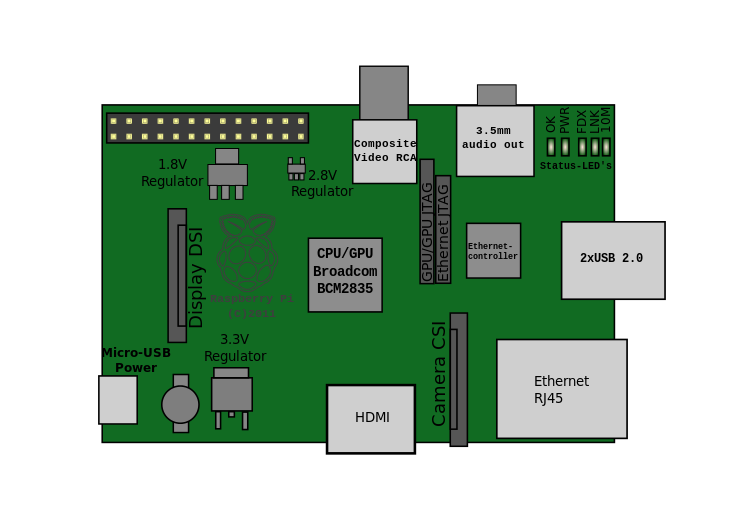
\includegraphics[width=0.5\textwidth]{raspi_pcb}
  \label{fig:raspi_pcb}
\end{figure}

\subsubsection{Broadcom BCM2835 CPU y GPU}
\subsubsection{Memoria}
\subsubsection{GPIO (Entradas y salidas de prop�sito general)}

\begin{table}
\centering
  \begin{tabular}{r r r r}
\textbf{Pin} & \textbf{Descripci�n} & \textbf{Pin} & \textbf{Descripci�n} \\
\hline
1 & \texttt{3.3v} & 2 & \texttt{5v} \\
3 & \texttt{SDA0*} & 4 & \texttt{5v} \\
5 & \texttt{SCL0*} & 6 & \texttt{GND} \\
7 &  \texttt{GPIO\_GCLK} & 8 & \texttt{TXD0*} \\
9 &  \texttt{GND} & 10 & \texttt{RXD0*} \\
11 &  \texttt{GPIO\_GEN0} & 12 & \texttt{GPIO\_GEN1} \\
13 &  \texttt{GPIO\_GEN2} & 14 & \texttt{GND} \\
15 &  \texttt{GPIO\_GEN3} & 16 & \texttt{GPIO\_GEN4} \\
17 &  \texttt{3.3v} & 18 & \texttt{GPIO\_GEN5} \\
19 &  \texttt{SPI\_MOSI*} & 20 & \texttt{GND} \\
21 &  \texttt{SPI\_MISO*} & 22 & \texttt{GPIO\_GEN6} \\
23 &  \texttt{SPI\_SCLK*} & 24 & \texttt{SPI\_CEO\_N*} \\
25 &  \texttt{GND} & 26 & \texttt{SPI\_CE1\_N*} \\
  \end{tabular}
  \caption{Descripci�n de los pines de GPIO}
  \label{table:gpio_descr}
\end{table}

\subsection{Modulo de C�mara}
\begin{figure}[h!]
  \caption{Modulo de c�mara de Raspberry Pi.}
  \centering
    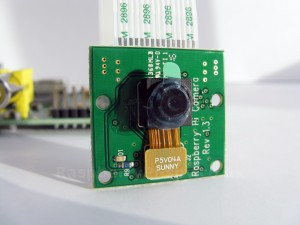
\includegraphics[width=0.5\textwidth]{raspi_camera}
  \label{fig:raspi_camera}
\end{figure}

\subsection{Software}
\section{Componentes el�ctricos, electr�nicos y electromec�nicos del Robot}
\subsection{Actuadores}
\subsubsection{Motores DC}
\subsection{Celdas 18650}
\subsubsection{Celdas Li-Ion}
\subsection{Regulador de voltaje}
\subsection{Controlador de motores DC}
Un ejemplo de funcionamiento del puente-en-H se muestra en la Figura~\ref{fig:h-bridge}, los interruptores S1, S2, S3 y S4 estan situados de tal manera que forman una letra H. \begin{figure}[h!]
  \caption{H-Bridge controlando un motor adelante y atras.}
  \centering
    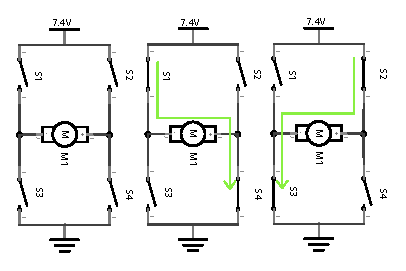
\includegraphics[width=0.4\textwidth]{h-bridge}
  \label{fig:h-bridge}
\end{figure}

\subsubsection{Puente-en-H dual L298}
El \texttt{L298} es un circuito integrado que contiene dos puentes-en-H, es decir que puede controlar dos motores al mismo tiempo. Este C.I. es capaz de controlar motores de alto voltaje y alta corriente, y acepta como entrada niveles logicos TTL.

\begin{figure}[h!]
  \caption{Empaquetado del circuito integrado L298}
  \centering
    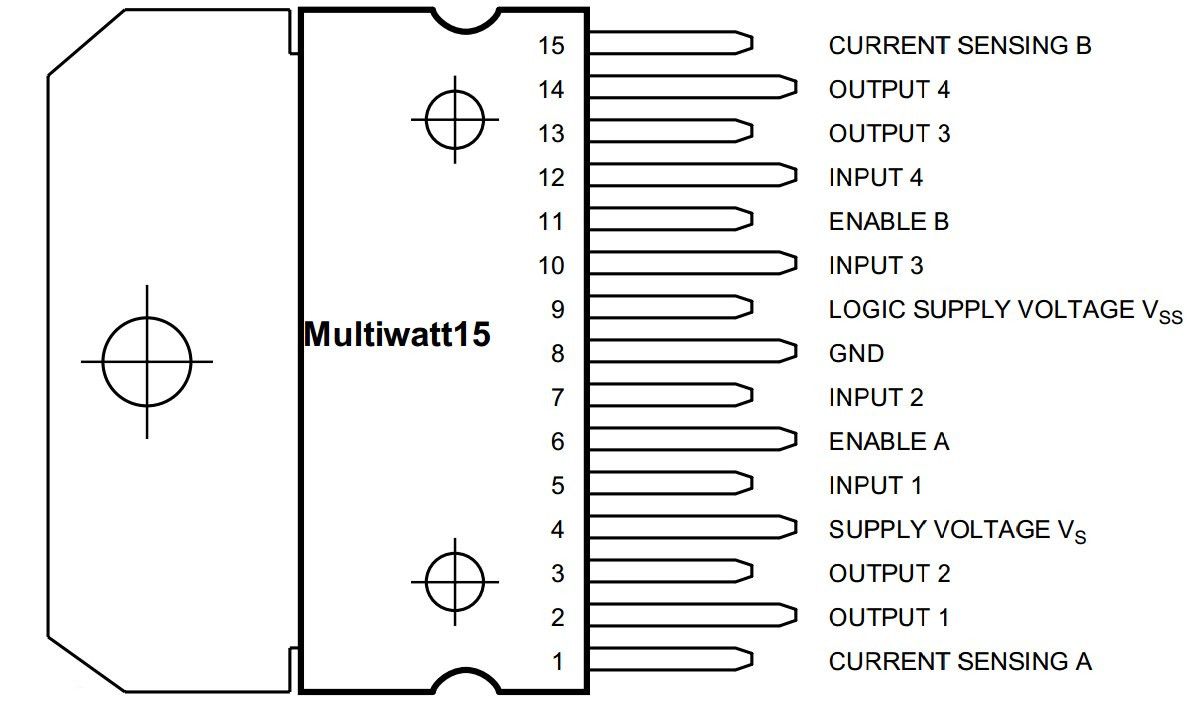
\includegraphics[width=0.4\textwidth]{hbci}
  \label{fig:hbci}
\end{figure}


%\subsection{}
%\subsection{}
\section{Partes mec�nicas del Robot}
\subsection{Tractor oruga}
\begin{figure}[h!]
  \caption{Ruedas y orugas Tamiya.}
  \centering
    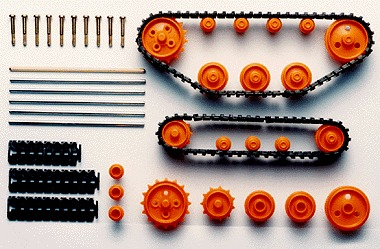
\includegraphics[width=0.4\textwidth]{oruga}
  \label{fig:oruga}
\end{figure}


\subsection{Chasis del Robot}
\subsection{Caja para celdas 18650}
%herramientas utlizadas
%descripcion de pines
%circuitos

% GPIO 18 servomotor
